\documentclass[11pt,letterpaper,titlepage]{article}

%================== Document nomenclature
\newcommand{\DOCSUBJT}{Whitepaper: }   %Put document subject here
\newcommand{\DOCTITLE}{                      %Put document title here
	Diffusion Solver in ChiTech
}       
\newcommand{\DOCDATE} {August, 2018}         %Put document date here
\newcommand{\DOCREV}  {Rev 1.00}             %Put revision number here

%================== Misc Settings
\usepackage{fancyhdr}
\usepackage[left=0.75in, right=0.75in, bottom=1.0in]{geometry}
\usepackage{lastpage}
\usepackage{titleref}
\usepackage{booktabs}
\usepackage{appendix}
\usepackage{ stmaryrd }

\appendixtitleon
\appendixtitletocon

\makeatletter

%================== List of figures and tables mods
\usepackage{tocloft}
\usepackage[labelfont=bf]{caption}

\renewcommand{\cftfigpresnum}{Figure\ }
\renewcommand{\cfttabpresnum}{Table\ }

\newlength{\mylenf}
\settowidth{\mylenf}{\cftfigpresnum}
\setlength{\cftfignumwidth}{\dimexpr\mylenf+1.5em}
\setlength{\cfttabnumwidth}{\dimexpr\mylenf+1.5em}



%=================== Graphics
\usepackage{graphicx}
\usepackage[breakwords]{truncate}
\usepackage{float}
\usepackage{array}
\usepackage{amsmath}
\usepackage{mdframed}
\usepackage{fancyvrb}
\usepackage{float}
\usepackage{cancel}
\usepackage{amssymb}
\graphicspath{ {images/} }
\usepackage[usenames,dvipsnames,svgnames,table]{xcolor}
\usepackage[defaultlines=2,all]{nowidow}
\usepackage{listings}
\usepackage{color}
\definecolor{Brown}{cmyk}{0,0.81,1,0.60}
\definecolor{OliveGreen}{cmyk}{0.64,0,0.95,0.40}
\definecolor{CadetBlue}{cmyk}{0.62,0.57,0.23,0}
\usepackage{pdflscape}
\usepackage{relsize}
\usepackage{verbatim}
\usepackage{tabto}
\usepackage{upgreek}
\usepackage{enumitem}

\usepackage{mathtools}

%=================== Settings
\renewcommand{\baselinestretch}{1.2}
\definecolor{gray}{rgb}{0.4 0.4 0.4}
\newcommand{\stimes}{{\times}}

\newcommand*{\ldblbrace}{\{\mskip-5mu\{}
\newcommand*{\rdblbrace}{\}\mskip-5mu\}}


\newcommand{\xmltag}[1]{\textcolor{blue}{ \texttt{#1}} }
\newcommand{\xmloption}[1]{\textcolor{ao(english)}{ \texttt{#1}} }

%================== Code syntax highlighting
\lstset{language=C++,frame=ltrb,framesep=2pt,basicstyle=\linespread{0.8} \small,
	keywordstyle=\ttfamily\color{OliveGreen},
	identifierstyle=\ttfamily\color{CadetBlue}\bfseries,
	commentstyle=\color{Brown},
	stringstyle=\ttfamily,
	showstringspaces=true,
	tabsize=2,}

\newcommand{\bOmega}{\mathcal{D}}

%\setlength\parindent{0pt}

%================== Custom commands
\newcommand{\Omegabf}{\mathbf{\Omega}}
\newcommand{\position}{\mathbf{r}}


\newcommand{\beq}{\begin{equation*}
\begin{aligned}}
\newcommand{\eeq}{\end{aligned}
\end{equation*}}

\newcommand{\beqn}{\begin{equation}
	\begin{aligned}}
\newcommand{\eeqn}{\end{aligned}
	\end{equation}}

\newcommand{\bnabla}{\boldsymbol{\nabla}}
\newcommand{\bvel}{\mathbf{u}}
\newcommand{\pluseq}{\mathrel{+}=}
\newcommand{\asteq}{\mathrel{*}=}

%=================== Big cdot
\newcommand*\bigcdot{\mathpalette\bigcdot@{.5}}
\newcommand*\bigcdot@[2]{\mathbin{\vcenter{\hbox{\scalebox{#2}{$\m@th#1\bullet$}}}}}

%================== Section numbers with equation numbers
\numberwithin{equation}{section}

\begin{document}

\begin{titlepage}
	\pagestyle{fancy}
	\vspace*{1.0cm}
	\centering
	\vspace{1cm}
	\vspace{.25cm}
	{\Large\bfseries  \DOCSUBJT \par} 
	{\Large\bfseries \DOCTITLE  \par}
	\vspace{1cm}
	{\Large \DOCDATE \par}
	\vspace{1.0cm}
	{\Large Jan Vermaak \par}
	{\Large \DOCREV \par}
	\begin{center}
		\begin{minipage}[c]{0.45\textwidth}
			\begin{figure}[H]
				
				\includegraphics[width=3in]{Logo2_Medium.png}
			\end{figure}
		\end{minipage}
	\end{center}

\end{titlepage}	


\pagestyle{fancy}
\rfoot{Page \thepage \ of \pageref{LastPage}}
\cfoot{}
\lfoot{\truncate{14cm}{\DOCTITLE}}
\rhead{}
\chead{\currentname}
\lhead{}
\renewcommand{\footrulewidth}{0.4pt}


\tableofcontents
\addtocontents{toc}{~\hfill\textbf{Page}\par}
%
%\listoffigures
%\listoftables


%#########################################################################
\chead{Introduction}
\newpage
\section{Introduction}
The ``generalized diffusion solver" in Chi-Tech is based on a well known partial differential equation known as the \textbf{diffusion equation}. This equation can be used to model the behavior of many physical systems and has been studied in great depth for many years by engineers, scientists and mathematicians. The equation for a single unknown, $\phi$, has the general time dependent linear form

\begin{equation} \label{eq:general_diffeq}
\frac{d\phi}{dt} = \bnabla \cdot (D\bnabla\phi) - \sigma \phi + q
\end{equation}
\newline
and can be outfitted with a number of different boundary conditions including Dirichlet-type, Neumann-type, and Robin-type boundary conditions.
Different spatial discretizations can be applied to the equation including Finite Difference (FD), Finite Volume (FV), Continuous Galerkin Finite Element Method (CFEM), and Discontinuous Galerkin Finite Element (DFEM). In Chi-Tech the available spatial discretizations are FV, CFEM and DFEM. Additionally, different time discretizations can be applied for which Chi-Tech for now supports Forward Euler, Backward Euler, and Crank-Nicholson.

The steady state form of the diffusion equation will be used in this whitepaper to detail the different spatial discretization techniques and is denoted by

\begin{equation} \label{eq:steady_diffeq}
-\bnabla \cdot (D\bnabla\phi) + \sigma \phi = q.
\end{equation}
\newline
This equation can be related to techniques contained in literature under certain conditions. When the removal term ($\sigma \phi$) is removed and $D{=}1$ then the equation becomes Poisson's equation 

\begin{equation} \label{eq:poisson_eq}
\bnabla \cdot (\bnabla\phi) = -q,
\end{equation}
\newline
and if the spatial source term, $q$, is also removed then the equation becomes Laplace's equation

\begin{equation} \label{eq:laplace_eq}
\bnabla \cdot (\bnabla\phi) = 0.
\end{equation}
\newline 
In both these forms the divergence of the gradient ($\bnabla\cdot\bnabla\phi$) is replaced by the Laplacian operator, $\bnabla^2$, which can generally denoted by the symbol $\Delta$ after which the following are equivalent 

\begin{equation}
\begin{aligned}
\bnabla\cdot\bnabla\phi &= 0 \\ 
\bnabla^2 \phi &=0 \\
 \Delta\phi &= 0
\end{aligned}
\end{equation} 


\newpage
\chead{Finite Volume}
\section{Finite Volume}
\subsection{Discretization}
The FV method associates only a single value of the unknown per cell, located at the cell centroid, and is discretized by first integrating equation \eqref{eq:steady_diffeq} over the cell volume

\begin{equation}
\begin{aligned}
-\int_V \bnabla \cdot (D\bnabla\phi) \ dV + \int_V \sigma \phi \ dV = \int_V q \ dV
\end{aligned}
\end{equation}
\newline
after which we apply Gauss' divergence theorem to the first term

\begin{equation}
\begin{aligned}
-\int_V \bnabla \cdot (D\bnabla\phi) \ dV = 
-\int_S \mathbf{n} \cdot (D\bnabla\phi) \ dA
\end{aligned}
\end{equation}
\newline 
and then apply discretized integration over cell volume, $V$, and cell face areas, $A_f$,

\begin{equation}\label{eq:fv_needface}
\begin{aligned}
-\sum_f \mathbf{A}_f \cdot (D\bnabla\phi)_f  + V (\sigma \phi) = V \ q,
\end{aligned}
\end{equation}
\newline 
where $\mathbf{A}_f = A_f \mathbf{n}_f$ is the face area vector. This formulation is not complete until we have a discretized expression for $(D\bnabla \phi)_f$. The problem in depicting the details of this term in a Finite Volume discretization scheme is that it has a tremendously simplistic representation on orthogonal grids, and a significantly more complicated representation in unstructured grids. Generally the prior (on orthogonal grids) exhibits 2nd order convergence, however, the latter requires more care because the possibility of skewed faces can cause the method to become less than 1st order accurate.
\newline
\newline 
The next two sections are devoted to separately describe the discretization on orthogonal and unstructured grids, respectively. Ultimately the unstructured implementation will be used since it is unifying, however, the general process can be observed on the orthogonal grid detail.

\newpage 
\subsection{Discretization on Orthogonal grids}
\subsubsection{Terminology}
Figure \ref{fig:orthogonalgridfv} below contains a graphic depiction of orthogonal 2D cells which we will use the define numerous concepts.

\begin{figure}[H]
\centering
\includegraphics[width=0.3\linewidth]{Figures/OrthogonalGridFV}
\caption{Reference vector layout for neighboring cells on an orthogonal grid.}
\label{fig:orthogonalgridfv}
\end{figure}
\noindent
The points $\mathbf{P}$, $\mathbf{N}$ and $\mathbf{F}$ are the present-cell-, neighboring-cell- and adjoining-face-centroids, respectively. The vector $\mathbf{PF}$ is from $\mathbf{P}$ to $\mathbf{F}$ and its length is used as $d_{PF}$. Similarly the vector $\mathbf{PN}$ is used to define $d_{PN}$.

\subsubsection{Weighted harmonic mean of a quantity $D$ at a face}
Some quantities, like the diffusion coefficient, require the harmonic mean at the faces. For orthogonal grids this requires a weighted harmonic mean where the weight requires the definition of
\beqn 
r_O = \frac{d_{PF}}{d_{PN}}
\eeqn 
after which the harmonic mean is defined as
\beqn
D_f = \biggr( 
\frac{r_O}{D_P} + 
\frac{1-r_O}{D_P}
\biggr)^{-1}
\eeqn 

\subsubsection{Flux of a gradient}
With the definition of face diffusion coefficient the required term in equation \eqref{eq:fv_needface} becomes

\beqn \label{eq:flux_of_gradient_ortho}
\mathbf{A}_f \bigcdot (D\bnabla \phi)_f = 
D_f\frac{A_f}{d_{PN}} 
\biggr(
\phi_N - \phi_P
\biggr)
\eeqn 

\subsubsection{Assembling the linear system}
We now proceed by inserting eq. \eqref{eq:flux_of_gradient_ortho} into eq. \eqref{eq:fv_needface}, and mark values at iteration $(n)$ to be implicit and values at $(n-1)$ as explicit,  to get

\beqn
-\sum_fD_f\frac{A_f}{d_{PN}} 
\biggr(
\phi_N - \phi_P
\biggr)^{(n)}  + V \sigma \phi_P^{(n)} = V \ q_P^{(n-1)}
\eeqn 

\noindent 
This can then be simplified into a coefficient formulation

\beq 
a_P \phi_P + \sum_f a_{Nf} \phi_N = b_N
\eeq 
\newline 
where 
\beq 
a_P &= \sum_f D_f\frac{A_f}{d_{PN}}   + V \sigma \\
a_{Nf} &= -D_f\frac{A_f}{d_{PN}} \\
b_N &= V \ q_P^{(n-1)}
\eeq 
\newline 
\noindent 
The final process is to assemble this coefficient formulation for each cell $P$ where each index $N$ and $P$ maps to a given $i,j$ matrix or $i$ vector index. The methodology to obtain these $i,j$ indices requires some machinery to be developed relating to sparsity patterns which will be discussed next.


\newpage 
\subsection{Discretization on Unstructured grids}
\subsubsection{Terminology}

Figure \ref{fig:faceaverages} below contains a graphic depiction of unstructured 2D cells which we will use to define numerous concepts.

\begin{figure}[H]
\centering
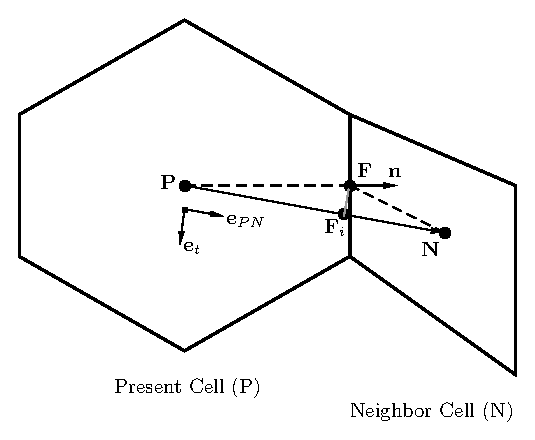
\includegraphics[width=0.5\linewidth]{Figures/FaceAverages}
\caption{Reference vector layout for neighboring cells on an unstructured grid.}
\label{fig:faceaverages}
\end{figure}
\noindent
The points $\mathbf{P}$, $\mathbf{N}$ and $\mathbf{F}$ are the present-cell-, neighboring-cell- and adjoining-face-centroids, respectively. The vector $\mathbf{PN}$ is from $\mathbf{P}$ to $\mathbf{N}$, and the projection of $\mathbf{PF}$ onto $\mathbf{PN}$ is at point $\mathbf{F}_i$ (not actually at the intersection of $\mathbf{PN}$ with the face). The vector $\mathbf{e}_{PN}$ is the unit vector along $\mathbf{PN}$ computed from $\mathbf{PN}/d_{PN}$, where $d_{PN} = || \mathbf{PN} ||_2$. The vector $\mathbf{e}_t$ is the unit tangential vector formed from $\mathbf{e}_t = \mathbf{e}_{PN} - \mathbf{n}$, with $\mathbf{n}$ being the face normal. The distance from $\mathbf{P}$ to $\mathbf{F}_i$, $d_{PF_i}$, is computed as 
$
d_{PF_i} = \mathbf{PF} \ \bigcdot  \ \mathbf{e}_{PN}
$, 
and $\mathbf{F}_i = \mathbf{P} + d_{PF_i}  \ \mathbf{e}_{PN}$.

%
%\subsubsection{Linear interpolation of a quantity $\phi$ to a face, option 1}
%A linear interpolation of any quantity $\phi$, to find $\phi_{f_i}$, can be determined by defining 
%\beqn 
%r_P = \frac{d_{PF_i}}{d_{PN}}
%\eeqn 
%from which 
%\beqn \label{eq:linear_interpolation_nocorr}
%\phi_{f_i} &= (1-r_P) \phi_P + (r_P)\phi_N.
%\eeqn
%This is however not the desired value at the cell centroid, i.e. $\phi_f$. To correct for this we can linearly interpolate the gradient of $\phi$ to $\mathbf{F}_i$ and extend towards $\mathbf{F}$ as
%\beq 
%\bnabla \phi_{f_i} = (1-r_P) \bnabla \phi_P + (r_P)\bnabla \phi_N
%\eeq 
%using the vector from $\mathbf{F}_i$ to $\mathbf{F}$, $\mathbf{F_iF}$, to get
%\beqn \label{eq:linear_interpolation}
%\phi_f \approx \phi_{f_i}
%+ \bnabla \phi_{f_i} \bigcdot \mathbf{F_iF}
%\eeqn
%which can be used for the interpolation of the pressure and/or temperature. Note however, that this form is not suitable for the interpolation of the velocity, which requires special treatment.
%
%\subsubsection{Linear interpolation of a quantity $\phi$ to a face, option 2}
%For quantities that are not very sensitive to variation in the direction of the face skewness,  one can apply a less accurate, but still suitable interpolation, by neglecting the gradients and using the normal distance to the face. This requires $r_f$ defined as
%\beqn 
%r_f = \frac{
%\mathbf{PF} \bigcdot \mathbf{n}
%}{
%\mathbf{PF} \bigcdot \mathbf{n} +
%\mathbf{FN} \bigcdot \mathbf{n}
%}
%\eeqn 
%
%which can then be used to linearly interpolated quantities as
%\beqn \label{eq:linear_interpolation_nocorr2}
%\phi_{f_i} &= (1-r_f) \phi_P + (r_f)\phi_N.
%\eeqn

\subsubsection{Weighted harmonic mean of a quantity $D$ at a face}
Some quantities, like the diffusion coefficient, require the harmonic mean at the faces. For unstructured grids this requires a weighted harmonic mean where the weight requires the definition of
\beqn 
r_P = \frac{d_{PF_i}}{d_{PN}}
\eeqn 
after which the harmonic mean is defined as
\beqn
D_f = \biggr( 
\frac{r_P}{D_P} + 
\frac{1-r_P}{D_P}
\biggr)^{-1}
\eeqn 


\vspace{0.5cm}
\subsubsection{Flux of a gradient}
We can now develop the computation of $\mathbf{A}_f \bigcdot (D_f \bnabla \phi)_f$. When we deal with skewed faces, this diffusion  term needs some treatment. In general, since the face is skewed, the flux at the cell face develops additional components other than the orthogonal component along the direction of $\mathbf{PN}$.  These additional components are not intuitive to understand. Refer to Figure \ref{fig:faceaveragesskewed} below for the following discussion.

\begin{figure}[H]
\centering
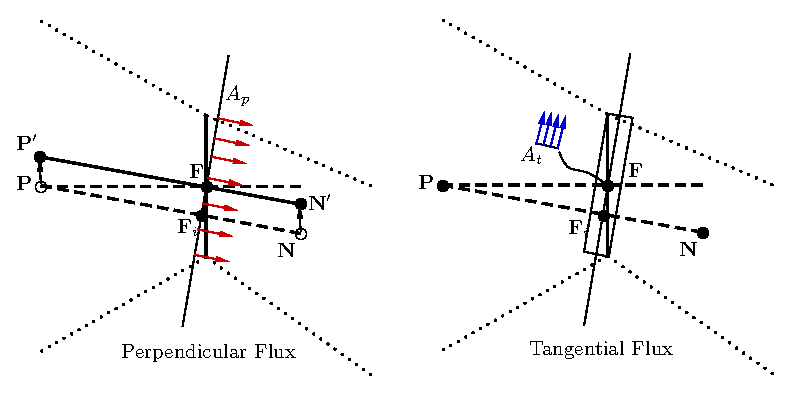
\includegraphics[width=0.8\linewidth]{Figures/FaceAveragesSkewed}
\caption{Decomposed areas for the interpolation of a gradient flux}
\label{fig:faceaveragesskewed}
\end{figure}

Given that the correct way to approximate the flux across the face is to compute the gradient along its centroid, we require the gradient to be computed from $\phi_{P'}$ and $\phi_{N'}$ along the projected perpendicular area $A_p$. Additionally we need to compute the flux along the tangential area $A_t$. Including these terms within an implicit formulation is, however, cumbersome to say the least. Instead we include explicit corrections as described in \cite{Sezai}.
\newline
\newline
Firstly, we formulate the fluxes at $\mathbf{P}'$ and $\mathbf{N}'$ (see the left schematic in Figure \ref{fig:faceaveragesskewed}) as 

\beqn 
\phi_{P'} &= \phi_P + (\bnabla \phi)_P^{(n-1)} \  \bigcdot  \ \mathbf{F_iF} \\
\phi_{N'} &= \phi_N + (\bnabla \phi)_N^{(n-1)} \  \bigcdot \  \mathbf{F_iF}
\eeqn 
\newline
where $\mathbf{F_iF}$ is the vector from $\mathbf{F}_i$ to $\mathbf{F}$ and the gradients are computed from the previous iteration's flux field. The perpendicular gradient term can then be computed from

\beq 
\biggr (
\mathbf{A}_f \bigcdot (\bnabla \phi)_f 
\biggr)_p
&=
\frac{A_p}{d_{PN}} \biggr ( \phi_{N'} - \phi_{P'} \biggr)
\\
&= \frac{A_p}{d_{PN}} \biggr ( \phi_{N} - \phi_{P} \biggr)
+  \frac{ A_p }{d_{PN}} \biggr ( (\bnabla \phi)_N  -  (\bnabla \phi)_P \biggr)^{(n-1)}
\ \bigcdot \mathbf{F_iF} 
\eeq 
\newline 
where $A_p = A_f / (\mathbf{e}_{PN} \bigcdot \mathbf{n})$. Secondly, the tangential component can be computed from 

\beqn 
\biggr (
\mathbf{A}_f \bigcdot (\bnabla \phi)_f 
\biggr)_t
&= (\bnabla \phi)_F \bigcdot \mathbf{A}_t
\\
&\approx  (\bnabla \phi)_{F_i}^{(n-1)} \bigcdot \mathbf{A}_t
\eeqn 
\newline
where $\mathbf{A}_t = \mathbf{A}_f - A_p \mathbf{e}_{PN}$ and the gradient at the face centroid is approximated by the gradient interpolated at $\mathbf{F}_i$ which is not an unreasonable approximation considering that cell skewness is normally minimized. 
Putting it all together we have

\beqn \label{eq:flux_of_gradient}
\mathbf{A}_f \bigcdot (\bnabla \phi)_f 
=
 \frac{A_p}{d_{PN}} \biggr ( \phi_{N} - \phi_{P} \biggr)
+  \frac{ A_p }{d_{PN}} \biggr ( (\bnabla \phi)_N  -  (\bnabla \phi)_P \biggr)^{(n-1)}
\ \bigcdot \mathbf{F_iF} 
+
 (\bnabla \phi)_{F_i}^{(n-1)} \bigcdot \mathbf{A}_t
\eeqn 
\newline
In these equations we require the explicit value of $(\bnabla \phi)^{n-1}$ which can be computed using different methods, i.e., Green-Gauss and Weighted least-squares. These two methods will now be detailed.

\vspace{0.5cm}
\subsubsection{Computing gradients using Green-Gauss}

This formulation is identical to ``Option 3" of chapter 9.2 in the book by Moukalled et al. \cite{MMD}.
The first order Green-Gauss approximation reduces essentially to a summation over faces.

\beqn \label{eq:gradient_gg} 
\bnabla \phi = \frac{1}{V} \sum_f \mathbf{A}_f \phi_f
\eeqn 

where $\phi_f$ is taken as a linear interpolation between the adjoining face's cells. This formulation poses some challenges when undetermined faces fluxes are encountered, as is the case with boundaries and unstructured meshes, and therefore we require an algorithm to compensate. Therefore the following algorithm is applied:

\begin{enumerate}
\item Compute $\bnabla \phi^{(n)}$ over the entire domain using $\frac{1}{V}\sum_f \mathbf{A}_f \phi_f$ where $\phi_f$ is computed from \eqref{eq:linear_interpolation} as
\beq
\phi_f &= 
(1-r_P) \phi_P + (r_P)\phi_N + 
\biggr [
(1-r_P) \bnabla \phi_P + (r_P)\bnabla \phi_N
\biggr ]^{(n-1)} \bigcdot \mathbf{F_iF}
\eeq 
and boundary faces are computed as
\beq 
\phi_b = \phi_P + \bnabla \phi_P^{(n-1)} \bigcdot  \ \mathbf{PF}
\eeq 

\item Compute $|| \bnabla \phi^{(n)} - \bnabla \phi^{(n-1)} ||_2$. If $|| \bnabla \phi^{(n)} - \bnabla \phi^{(n-1)} ||_2<\epsilon$ then terminate.

\item Swap $\bnabla \phi^{(n)}$ and $\bnabla \phi^{(n-1)}$.
\item Repeat 2 to 4.
\end{enumerate}

In most cases the iteration process adds little to the iterative performance and it can be sufficient to just terminate after a single iteration.


\vspace{1cm}
\subsubsection{Computing gradients using weighted Least-Squares}
Section 9.3 in \cite{MMD} provides a very good description of how the weighted Least-Squares gradients are determined. In that formulation

\beq
\begin{Bmatrix}
\sum_f w_f \mathbf{PN} \otimes \mathbf{PN} 
\end{Bmatrix}
\bnabla \phi_P
=
\sum_f
\begin{bmatrix}
w_f \mathbf{PN} (\phi_N - \phi_P)
\end{bmatrix}
\eeq   
where
\beq 
w_f = \frac{1}{(|| \mathbf{PN} ||_2)^2}
\eeq 
and the term in $\{\}$ is a tensor. On boundaries, $\mathbf{PN}$ and $\phi_N$ is replaced by $\mathbf{PF}$ and $\phi_b$.
\newline
\newline
Note that this results in a system that needs to solved for each cell.

\vspace{0.5cm}
\subsubsection{Assembling the linear system}
With all the individual pieces of functionality established we can now determine how to assemble the linear system. We start with eq. \eqref{eq:fv_needface} where now we insert eq. \eqref{eq:flux_of_gradient}, and mark values at iteration $(n)$ to be implicit and values at $(n-1)$ as explicit, after which we get

\begin{equation}
\begin{aligned}
-\sum_f D_f \biggr[
\frac{A_p}{d_{PN}} \biggr ( \phi_{N} - \phi_{P} \biggr)^{(n)}
+  \frac{ A_p }{d_{PN}} \biggr ( (\bnabla \phi)_N  -  (\bnabla \phi)_P \biggr)^{(n-1)}
\ \bigcdot \mathbf{F_iF} 
+
 (\bnabla \phi)_{F_i}^{(n-1)} \bigcdot \mathbf{A}_t
 \biggr]
 + V \sigma \phi_P^{(n)} = V \ q_P^{(n-1)}
\end{aligned}
\end{equation}
\noindent
which we can arrange to have all the implicit values to the left

\begin{equation}
\begin{aligned}
-\sum_f D_f \biggr[
\frac{A_p}{d_{PN}} \biggr ( \phi_{N} - \phi_{P} \biggr)^{(n)}
 \biggr]
 + V \sigma \phi_P^{(n)} &= 
 V \ q_P^{(n-1)} \\
 &+
 \sum_f  D_f\biggr[
 \frac{ A_p }{d_{PN}} \biggr ( (\bnabla \phi)_N  -  (\bnabla \phi)_P \biggr)^{(n-1)}
 \ \bigcdot \mathbf{F_iF} 
 +
  (\bnabla \phi)_{F_i}^{(n-1)} \bigcdot \mathbf{A}_t
  \biggr].
\end{aligned}
\end{equation}
\noindent
This can be simplified into a coefficient formulation
\begin{equation}
\begin{aligned}
a_P \phi_P + \sum_f a_{Nf} \phi_N = b_N
\end{aligned}
\end{equation}
\noindent
where
\begin{equation} \label{eq:fv_coeffs}
\begin{aligned}
a_P &= \sum_f D_f \frac{A_p}{d_{PN}} + V\sigma \\
a_{Nf} &= -D_f \frac{A_p}{d_{PN}} \\
b_N &= V \ q_P^{(n-1)} 
 +
 \sum_f b_{Nf} \\
b_{Nf} &= D_f \biggr[
 \frac{ A_p }{d_{PN}} \biggr ( (\bnabla \phi)_N  -  (\bnabla \phi)_P \biggr)^{(n-1)}
 \ \bigcdot \mathbf{F_iF} 
 +
  (\bnabla \phi)_{F_i}^{(n-1)} \bigcdot \mathbf{A}_t
  \biggr].
\end{aligned}
\end{equation}
\newline
\noindent 
The final process is to assemble this coefficient formulation for each cell $P$ where each index $N$ and $P$ maps to a given $i,j$ matrix or $i$ vector index. The methodology to obtain these $i,j$ indices requires some machinery to be developed relating to sparsity patterns which will be discussed next.

\vspace{1cm}
\subsection{Boundary conditions}
\subsubsection{Dirichlet boundary conditions $\phi_N=\phi_B$}
A Dirichlet boundary condition manifests in the $\mathbf{A}_f \bigcdot (D\bnabla \phi)_f$ term where we start with

\beq 
\mathbf{A}_f \bigcdot (\bnabla \phi)_f 
=
 \frac{A_p}{d_{PN}} \biggr ( \phi_{N} - \phi_{P} \biggr)^{(n)}
+  \frac{ A_p }{d_{PN}} \biggr ( (\bnabla \phi)_N  -  (\bnabla \phi)_P \biggr)^{(n-1)}
\ \bigcdot \mathbf{F_iF} 
+
 (\bnabla \phi)_{F_i}^{(n-1)} \bigcdot \mathbf{A}_t
\eeq 
\newline
and note that the definition of $\mathbf{F_iF}$ requires the projection of $\mathbf{PF}$ onto $\mathbf{PN}$, however, in this case the vectors $\mathbf{PF}$ and $\mathbf{PN}$ are the same and therefore $\mathbf{F_i}$ equals $\mathbf{F}$ from which it follows that $\mathbf{F_iF}$ is zero in magnitude. We also know that $(\bnabla \phi)_{N}=0$ and therefore $ (\bnabla \phi)_{F_i}^{(n-1)}$ just becomes the projection of $(\bnabla \phi)_{P}$ to $\mathbf{F}$. Since  $(\bnabla \phi)_{P}$ is constant over the whole cell, $ (\bnabla \phi)_{F_i}^{(n-1)}$ is simply taken to be equal to $(\bnabla \phi)_{P}$ from which we now have

\beq 
\mathbf{A}_f \bigcdot (D\bnabla \phi)_f = 
 D_f \biggr[
 \frac{A_p}{d_{PN}} \biggr ( \phi_{B} - \phi_{P}^{(n)} \biggr) +
  (\bnabla \phi)_{P}^{(n-1)} \bigcdot \mathbf{A}_t
  \biggr]
\eeq 
\newline
\noindent 
Note the substitution of $\phi_N = \phi_B$, $D_f = D_P$, and the change to the iteration indices. This term then alters, for face $f^*$, the $a_{Nf}$ and $b_{Nf}$ coefficients in eq. \eqref{eq:fv_coeffs} as 

\beq 
a_{Nf^*} &= 0 \\
b_{Nf^*} & =  D_{f^*} 
\biggr[
\frac{A_p}{d_{PN}} \phi_B + 
(\bnabla \phi)_{P}^{(n-1)} \bigcdot \mathbf{A}_t
\biggr] 
\eeq 

\vspace{0.5cm}
\subsubsection{Neumann boundary conditions $\mathbf{A}_f \cdot (D\boldsymbol{\nabla} \phi)_f = F$}
This type of a boundary condition specifies an area flux on face $f^*$ and reduces simply to the modifications

\beq 
a_P &= \sum_{\substack{f \\ f\ne f^*}} D_f \frac{A_p}{d_{PN}} + V\sigma\\
a_{Nf^*} &= 0 \\
b_{Nf^*} &= F
\eeq 

\vspace{0.5cm}
\subsubsection{Robin boundary conditions $a\phi + b\mathbf{A}_f \cdot (D\boldsymbol{\nabla} \phi)_f = F$}
A Robin-type boundary condition is a combination of a Dirichlet boundary condition and a Neumann boundary condition. It can be incorporated in the form

\beq 
\mathbf{A}_f \cdot (D\boldsymbol{\nabla} \phi)_f = \frac{F}{b} - \frac{a}{b} \phi_P
\eeq 
\newline 
which requires the coefficients in \eqref{eq:fv_coeffs} to be altered, for face $f^*$, as

\beq 
a_P &= \sum_{\substack{f \\ f\ne f^*}} D_f \frac{A_p}{d_{PN}} + V\sigma + \frac{a}{b}\\
a_{Nf} &= 0 \\
b_{Nf} &= \frac{F}{b}
\eeq 

\newpage
\subsection{Sparsity pattern}
\subsubsection{Base block}
The parallel sparsity pattern for matrix assembly requires \textbf{node ordering} in a single block-sense (base block) as depicted in Figure \ref{fig:discretizationbaseblockfv} below. The nodes are cell centered and the base blocks are dependent on the number of cells. The local base block size (i.e., number of entries) is the number of local cells and the global base block size is the total number of cells (globally). 
\vspace{0.5cm}
\begin{lstlisting}
auto fv = new SpatialDiscretization_FV;
spatial_discretization = fv;

fv->AddViewOfLocalContinuum(grid);
fv->AddViewOfNeighborContinuums(grid);
fv->ReOrderNodes(grid);
\end{lstlisting}
\vspace{0.5cm}
After nodal reordering all partition locations will have two populated arrays, \xmltag{locJ\_block\_address} and \xmltag{locJ\_block\_size}, indexed by partition-id (i.e., processor 15: \xmltag{locJ\_block\_address[15]} ). 

The \xmltag{locJ\_block\_address} array contains the global address where each partition's base block starts and the \xmltag{locJ\_block\_size} array contains each partitions base block size.

\begin{figure}[H]
\centering
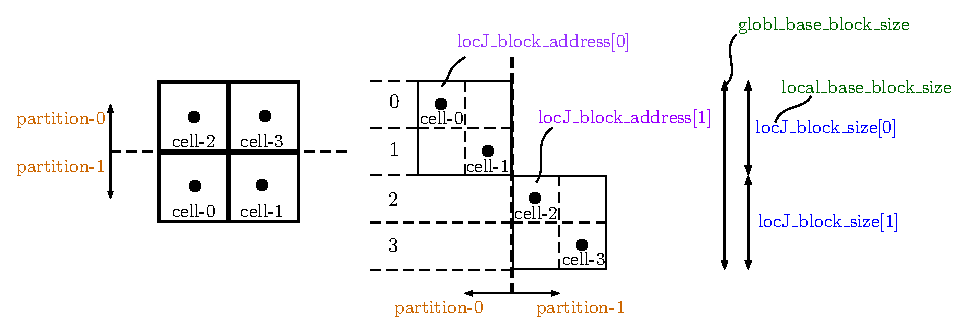
\includegraphics[width=0.9\linewidth]{Figures/DiscretizationBaseBlockFV.eps}
\caption{Base block node ordering for the Finite Volume discretization method.}
\label{fig:discretizationbaseblockfv}
\end{figure}

\subsubsection{Multiblock}
For mutliple degrees-of-freedom per node Chi-Tech supports two storage modes: Nodal and Block. Nodal-storage creates a block of unknowns per node, i.e., given a node address, the DOF-addresses will follow sequentially for each unknown. In contrast, Block-storage creates a block for each unknown, i.e., each block contains all the nodes but only a single unknown. The addressing scheme is determined as shown in Figure \ref{fig:discretizationcomponentblockfv} below which depicts 3 unknown (DOFs) per node. The color coding blue, green and red denotes the particular unknown, i.e., \textit{Velocity-x,y,z}, or \textit{Groups 0,1,2}.

\begin{figure}[H]
\centering
\includegraphics[width=1.0\linewidth]{Figures/DiscretizationComponentBlockFV}
\caption{Addressing scheme for multiblock unknowns with the Finite Volume discretization method.}
\label{fig:discretizationcomponentblockfv}
\end{figure}


\newpage
\chead{Continuous Finite Element Method}
\section{Continuous Finite Element Method}
\subsection{Discretization}
\subsubsection{Weak form}
As a preface to the spatial discretization using CFEM and DFEM we first introduce the general weak form of the diffusion equation. We proceed with multiplying with $\varphi_i$, a function mapping eq. \eqref{eq:general_diffeq} to a trial space $\mathcal{D}_i$ for which we require that

\begin{equation} \label{eq:trial}
\int_{\bOmega_i} \biggr( 
-\varphi_i\bnabla \bigcdot (D\bnabla\phi) 
\biggr).dV 
+ \int_{\bOmega_i} ( 
\varphi_i\sigma_a  \phi 
  ).dV
= \int_{\bOmega_i} (\varphi_i q).dV.
\end{equation}
\newline
In this equation we note that, from the product rule we have

\begin{align*}
\frac{d(fg)}{dx} &= \frac{df}{dx}\cdot g + f\cdot \frac{dg}{dx} \\
\therefore 
\int \frac{d(fg)}{dx} .dx&= \int \frac{df}{dx}\cdot g.dx + 
\int f\cdot \frac{dg}{dx}.dx
\end{align*}
\newline
Applying this as an analogy with $f=\varphi$ and $g=D\bnabla \phi$ we get the ``integration by parts" formulation 

\begin{equation}\label{eq:IntegrateByParts}
\begin{aligned}
\int_{\bOmega_i} \bnabla \bigcdot ( \varphi_i D\bnabla \phi) .dV&=
\int_{\bOmega_i} \bnabla \varphi_i\bigcdot D\bnabla \phi.dV + 
\int_{\bOmega_i} \varphi_i \bnabla \bigcdot (D\bnabla \phi).dV \\
\therefore
-\int_{\bOmega_i} \biggr(
\varphi_i \bnabla \bigcdot (D\bnabla \phi).dV
\biggr) &=
\int_{\bOmega_i} \bnabla \varphi_i \bigcdot D\bnabla \phi.dV
-\int_{\bOmega_i} \bnabla \bigcdot ( \varphi_i D\bnabla \phi) .dV
\end{aligned}
\end{equation}
\newline
Now applying Gauss's Divergence theorem on the last term we have
\begin{align}\label{eq:GaussDiv}
\int_{\bOmega_i} \bnabla \bigcdot ( \varphi_i D\bnabla \phi) .dV &=
\int_{\partial \bOmega} \mathbf{n}\cdot \varphi_i D\bnabla \phi . dA
\end{align}
\newline
which we can place in equation \ref{eq:IntegrateByParts} and then subsequently into equation \ref{eq:trial} which leads to the weak form

\begin{align}\label{eq:weakform}
\Aboxed{
\int_{\bOmega_i} \biggr(
\bnabla \varphi_i\bigcdot D\bnabla \phi
+
\varphi_i\sigma_a  \phi 
\biggr).dV 
- 
\int_{\partial \bOmega}\biggr( 
\mathbf{n}\cdot \varphi_i D\bnabla \phi 
\biggr). dA
= \int_{\bOmega_i} (\varphi_i q).dV
}.
\end{align}

\newpage
\subsubsection{Application of basis functions}
Consider $\phi$ approximated by the contributions of basis functions, $N_j$, and associated coefficients $\phi_j$, i.e.
\begin{align}
\phi \approx \phi_h = \sum_{j=0}^N \phi_j N_j.
\end{align}
Also consider the source $q$ as being a combination of: a constant-per-element component, $q_c$, and a non-constant-per-element component, $q_{nc}$. The non-constant component can then also be expandedusing basis functions and coefficients
\begin{align}
q_{nc} \approx q_{nc,h} = \sum_{j=0}^N q_{nc,j} N_j.
\end{align}
\newline
Equation \ref{eq:weakform} now becomes 

\begin{align*}
\begin{aligned}
&\int_{\bOmega_i} \biggr(
\bnabla \varphi_i\bigcdot D\bnabla (\sum_{j=0}^N \phi_j N_j)
+
\varphi_i\sigma_a  (\sum_{j=0}^N \phi_j N_j)
\biggr).dV
-
\int_{\partial \bOmega}\biggr( 
\mathbf{n}\bigcdot \varphi_i D\bnabla (\sum_{j=0}^N \phi_j N_j) 
\biggr). dA
\\
&= \int_{\bOmega_i} \varphi_i q_c.dV + \int_{\bOmega_i} \varphi_i (\sum_{j=0}^N q_{nc,j} N_j).dV 
\end{aligned}
\end{align*}
\noindent after which we can move the $\nabla$ operator such that
\begin{align*}
\begin{aligned}
&\int_{\bOmega_i} \biggr(
\bnabla \varphi_i\bigcdot D (\sum_{j=0}^N \phi_j \bnabla N_j)
+ 
\varphi_i\sigma_a  (\sum_{j=0}^N \phi_j N_j)
\biggr).dV
-
\int_{\partial \bOmega}\biggr( 
\mathbf{n}\bigcdot \varphi_i D (\sum_{j=0}^N \phi_j \bnabla N_j) 
\biggr). dA 
\\
&= \int_{\bOmega_i} \varphi_i q_c.dV+
 \int_{\bOmega_i} \varphi_i (\sum_{j=0}^N q_{nc,j} N_j).dV 
\end{aligned}
\end{align*}
\newline
We now take into account that each integral over a trial space $\bOmega_i$ is a summation over all the elements $\mathcal{K}$ that fall within this space. I.e.
\newline
\newline
\textbf{Trial space i}

\begin{equation*}
\begin{aligned}
&\sum^K \biggr[
\int_{\bOmega_i} \biggr(
\bnabla \varphi_i\bigcdot D (\sum_{j=0}^N \phi_j \bnabla N_j)
+
\varphi_i\sigma_a  (\sum_{j=0}^N \phi_j N_j)
\biggr).dV
-
\int_{\partial \bOmega}\biggr( 
\mathbf{n}\bigcdot \varphi_i D (\sum_{j=0}^N \phi_j \bnabla N_j) 
\biggr). dA \biggr]
\\
&=\sum^K \biggr[
 \int_{\bOmega_i} (\varphi_i q_c).dV
 +
  \int_{\bOmega_i} \varphi_i (\sum_{j=0}^N q_{nc,j} N_j).dV 
  \biggr]
\end{aligned}
\end{equation*}
Rearranging
\begin{equation*}
\begin{aligned}
&\sum^K
\sum_{j=0}^N
 \biggr[
\int_{\bOmega_i} \biggr(
\bnabla \varphi_i\bigcdot D ( \phi_j \bnabla N_j)
+
\varphi_i\sigma_a  ( \phi_j N_j)
\biggr).dV
-
\int_{\partial \bOmega}\biggr( 
\mathbf{n}\cdot \varphi_i D ( \phi_j \bnabla N_j) 
\biggr). dA \biggr]
\\
&=\sum^K 
\biggr[
 \int_{\bOmega_i} (\varphi_i q_c).dV
\biggr]
 +
 \sum^K
 \sum_{j=0}^N
 \biggr[
  \int_{\bOmega_i} \varphi_i ( q_{nc,j} N_j).dV 
  \biggr]
\end{aligned}
\end{equation*}

\begin{equation*}
\begin{aligned}
\therefore
&\sum^K
\sum_{j=0}^N \phi_j
 \biggr[ 
D \int_{\bOmega_i} 
\bnabla \varphi_i \bigcdot  \bnabla N_j.dV
+
\sigma_a \int_{\bOmega_i}  \varphi_i N_j
.dV
-
D \ \mathbf{n} \bigcdot \int_{\partial \bOmega}
 \varphi_i \bnabla N_j
. dA \biggr]
\\
&=\sum^K 
\biggr[q_c
 \int_{\bOmega_i} \varphi_i .dV 
 \biggr]
 +
 \sum^K
 \sum_{j=0}^N 
 \biggr[q_{nc,j}
  \int_{\bOmega_i} \varphi_i  N_j.dV 
  \biggr]
\end{aligned}
\end{equation*}
\newline
By using the same shape functions for the test functions as was used for the basis functions, $\varphi_i = N_i$, we have the following, Galerkin-form of the equations
\begin{equation}
\begin{aligned}
\therefore
&\sum^K
\sum_{j=0}^N \phi_j
 \biggr[ 
D \int_{\bOmega_i} 
\bnabla N_i \bigcdot  \bnabla N_j.dV
+
\sigma_a \int_{\bOmega_i}  N_i N_j
.dV
-
D \ \mathbf{n} \bigcdot \int_{\partial \bOmega}
 N_i \bnabla N_j
. dA \biggr]
\\
&=\sum^K 
\biggr[q_c
 \int_{\bOmega_i} N_i .dV 
 \biggr]
 +
 \sum^K
 \sum_{j=0}^N 
 \biggr[q_{nc,j}
  \int_{\bOmega_i} N_i  N_j.dV 
  \biggr]
\end{aligned}
\end{equation}
\newline
Computing the integrals of different combinations of the shape functions is specific to the type of element used, i.e. 1D slab, 2D triangle, 2D polygon, 3D tetrahedron, 3D polyhedron, etc. This information is contained in relevant whitepapers.

\subsubsection{Assembling the linear system of equations}
With each trial space representing an equation, we can assemble a row of a matrix $A$ and an associated entry in the vector $\mathbf{b}$ as
 
\vspace{0.25cm}
\textbf{For each element k, for each DOF-$i$, for each DOF-$j$}
\begin{equation}
\begin{aligned}
a_{ij} &=a_{ij} +  D \int_{\bOmega_i} \bnabla N_i  \cdot  \bnabla N_j .dV + 
\sigma_a \int_{\bOmega_i} N_i N_j.dV -
D \  \mathbf{n} \cdot \int_{\partial \bOmega} N_i  \bnabla N_j .dA 
\end{aligned}
\end{equation}
\begin{equation}
\begin{aligned}
b_i &= b_i 
+ q_{nc,j} \int_{\bOmega_i}  N_i  N_j .dV
\end{aligned}
\end{equation}

\textbf{For each element k, for each DOF-$i$}
\begin{equation}
\begin{aligned}
b_i &= b_i + q_c \int_{\bOmega_i} N_i   .dV 
\end{aligned}
\end{equation}

\subsection{Boundary conditions}
There are 2 primary types of boundary conditions implemented in ChiTech; \textbf{Dirichlet} type boundary conditions and \textbf{Robin} type boundary conditions.

\subsubsection{Robin and Neumann type boundary conditions}
A \textbf{Neumann} boundary condition takes the form

\begin{equation*}
-D \mathbf{n} \cdot \bnabla \phi = f \quad \quad \text{on } \partial \bOmega
\end{equation*}

where $f$ represents a function. This representation is trivial to implement in the equation for $a_{ij}$ since it essentially means the integral on the boundary is a known and can hence be moved to the right hand side. Hence the equations to do so simply become

\begin{equation*}
\begin{aligned}
a_{ij} &=a_{ij} +  D \int_{\bOmega_i} \bnabla N_i  \cdot  \bnabla N_j .dV + 
\sigma_a \int_{\bOmega_i} N_i N_j.dV - \cancel{
D \  \mathbf{n} \cdot \int_{\partial \bOmega} N_i  \bnabla N_j .dA} \\
b_i &= b_i 
+ q_{nc,j} \int_{\bOmega_i}  N_i  N_j .dV - f_j \int_{\partial\bOmega}  N_i  N_j .dA
\end{aligned}
\end{equation*}
and the rest remaining untouched.
\newline
\newline
In the case of a \textbf{Robin} boundary condition the form is similar;

\begin{equation*}
\alpha \phi+\beta D \mathbf{n} \cdot \bnabla \phi = f \quad \quad \text{on } \partial \bOmega
\end{equation*}

however, this time around there is a component still dependent on $\phi$ which must remain on the left hand side. The equations are

\begin{equation*}
\begin{aligned}
a_{ij} &=a_{ij} +  D \int_{\bOmega_i} \bnabla N_i  \cdot  \bnabla N_j .dV + 
\sigma_a \int_{\bOmega_i} N_i N_j.dV - \cancel{
D \  \mathbf{n} \cdot \int_{\partial \bOmega} N_i  \bnabla N_j .dA} 
+ 
\frac{\alpha}{\beta} \int_{\partial\bOmega} N_i N_j.dA\\
b_i &= b_i 
+ q_{nc,j} \int_{\bOmega_i}  N_i  N_j .dV + \frac{f_j}{\beta} \int_{\partial\bOmega}  N_i  b_j .dV
\end{aligned}
\end{equation*}
\newline
With this notation we can see that by using a Robin boundary condition with $\alpha=0$ and $\beta=-1$ we can essentially specify a Neumann boundary condition.
\newline
\newline
The versatility of this boundary condition can also be extended to \textbf{Vacuum} boundary conditions in neutron diffusion which take the form

\begin{equation*}
\frac{1}{4}\phi + \frac{1}{2}D\mathbf{n}\cdot\bnabla\phi = 0 \quad \quad \text{on } \partial \bOmega
\end{equation*}

representing a zero incoming current. It is simple to see that using the values $\alpha = \frac{1}{4}$, $\beta=\frac{1}{2}$ and $f=0$ one can specify a vacuum boundary condition using a Robin boundary condition.

\subsubsection{Dirichlet type boundary conditions}
The Robin type boundary conditions does not have the potential to destroy the symmetry of the matrix. \textbf{Dirichlet} boundary conditions on the other hand do have this potential. The Dirichlet boundary conditions takes the simple form

\begin{equation*}
\phi = c \quad \quad \text{on } \partial \bOmega.
\end{equation*}

Since none of the weak form equations have components of this form there is only one possible contribution to $a_{ij}$ and that is

\begin{equation*}
\begin{aligned}
&a_{ii} \mathbf{=} 1 \quad \quad a_{ij}=0\\
&b_i = c
\end{aligned}
\end{equation*}

Now, it is fairly trivial in theory to apply this process, however, with the finite element method normally assembling the matrix element-by-element the dirichlet boundary conditions will have to be applied after the element-by-element assembly. Additionally, the dirichlet process zeros out the non-diagonal columns of the given row. This is a problem because the rest of the element-by-element assembly connected other DOFs to the dirichlet DOF via the columns of their respective rows and hence if we do but zero out the non-diagonal components of the matrix row then we are left with a \textbf{non-symmetric} matrix.
\newline
\newline
In ChiTech the whole mess of Dirichlet boundary conditions is handled by modifying the element-by-element assembly process to never connect DOFs to the known dirichlet nodes. For a better understanding of how this is done please consult the coding implementation section.

\newpage
\subsection{Sparsity pattern}
\subsubsection{Base block}
Let us now consider a simple 2D arrangement of $4{\times}4$ cells as shown in Figure \ref{fig:fourbyfour} below. For a continuous finite element method the solution is defined on the nodes of the mesh whereas the cells are distributed on processors depicted with colors. This brings some choice on which processor will own a given node when shared.

\begin{lstlisting}
auto pwl = new SpatialDiscretization_PWL(0,
        chi_math::SpatialDiscretizationType::PIECEWISE_LINEAR_CONTINUOUS);
spatial_discretization = pwl;    

pwl->AddViewOfLocalContinuum(grid);
pwl->OrderNodesCFEM(grid);
\end{lstlisting}

\begin{figure}[H]
\centering
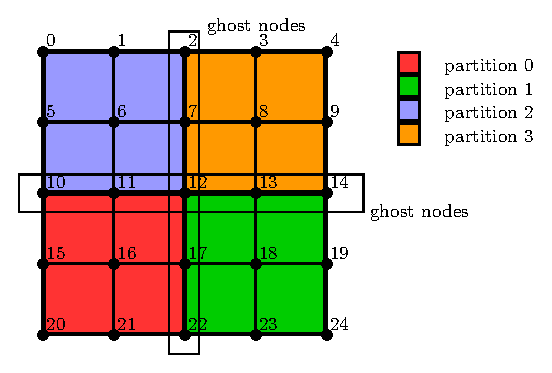
\includegraphics[width=0.5\linewidth]{Figures/DiscretizationBaseBlockCFEM.eps}
\caption{Simple CFEM arrangement of cells colored by processor ownership.}
\label{fig:fourbyfour}
\end{figure}
\noindent 
Nodal re-ordering is applied to the nodes of the mesh with a call to (\xmltag{ReorderNodesPWLC}). This process is a two stage process:
\newline
\newline
\textbf{Stage 1:}
\begin{itemize}
\item First all the nodes relevant to a process is collected into a set of exclusive and non-exclusive nodes. This involves a loop over all the nodes associated with a local cell.
\item Another loop is executed over local cells, however, this time we loop over faces and then face nodes. If a face is on a process boundary then node indices associated with all the face nodes are flagged as being ghosted.
\item Using the ghost flags, a list of exclusive nodes is creater as well as a list of non-exclusive nodes.
\item A ring communication is then used to communicate all the ghost nodes from location $i$ to location $i+1$ with the last location ending up with the complete list of ghost nodes. 
\item The last location then broadcasts the completed ghost node set to all other locations.
\end{itemize}

\textbf{Stage 2:}
\begin{itemize}
\item The ghost nodes are broken into $2P-2$ pieces (2 pieces per location, first and last locations get only 1 piece). If the amount of ghost nodes are not divisible they are stored as the remainder which will get subdivided between the first and last location.
\item With this information in hand each processor can determine the portion of the matrix it owns provided it knows the starting row. At this point only the first processor knows its ownership start ... its row 0. Therefore we initiate another ring communication. Each location takes its starting location, adds the local exclusive nodes, then the portion of the ghost nodes its been given and then sends the next location its starting location.
\item Perform the mapping of original node indexes to distributed node indices.
\end{itemize}

This process can be visualized as depicted in Figure \ref{fig:CFEMReordering} below. The ordering allows for minimal communication between processes and overall low bandwidth when the amount of rows per processor is small. If further bandwidth reduction is required then a suitable reordering is required per process to reorder the exclusive nodes.

\begin{figure}[H]
\centering
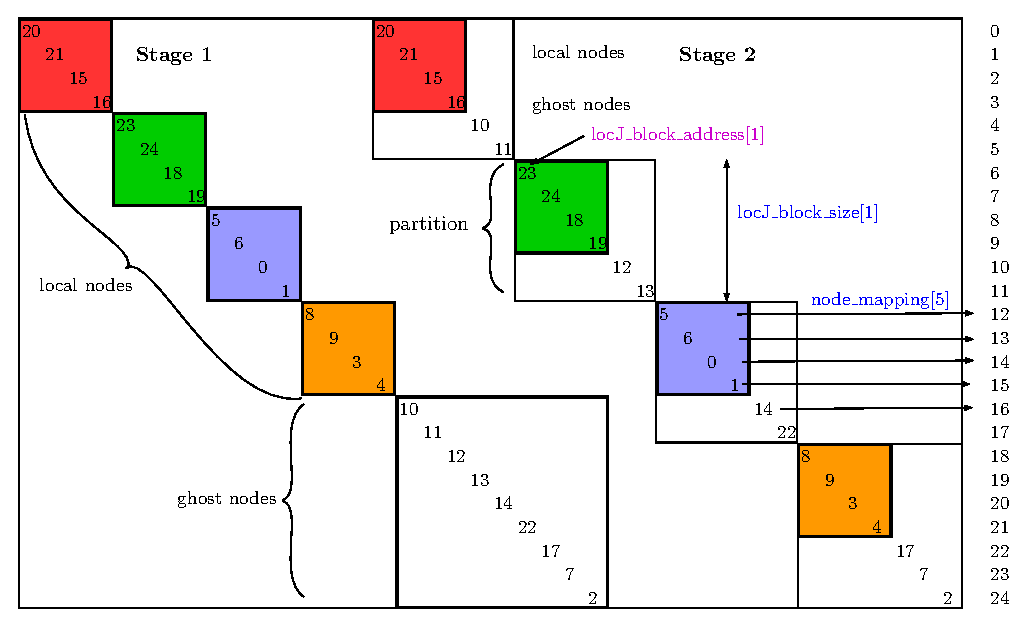
\includegraphics[width=0.95\linewidth]{Figures/DiscretizationBaseBlockCFEMStages.eps}
\caption{Stages of node ordering for CFEM.}
\label{fig:CFEMReordering}
\end{figure}

\noindent
After nodal reordering all partition locations will have three populated arrays, \xmltag{node\_mapping}, \xmltag{locJ\_block\_address} and \xmltag{locJ\_block\_size}. 

The \xmltag{node\_mapping} array maps a global node to the new parallel ordering and is indexed by node global id whereas the latter two are indexed by partition-id (i.e., processor 15: \xmltag{locJ\_block\_address[15]} ). 

The \xmltag{locJ\_block\_address} array contains the global address where each partition's base block starts and the \xmltag{locJ\_block\_size} array contains each partitions base block size.


\subsubsection{Multiblock}
For multiple degrees-of-freedom per node Chi-Tech support two storage modes: Nodal and Block. Nodal-storage creates a block of unknowns per node, i.e., given a node address, the DOF-addresses will follow sequentially for each unknown. In contrast, Block-storage creates a block for each unknown, i.e., each
block contains all the nodes but only a single unknown. Multiblock addressing is applied as shown

\begin{figure}[H]
\centering
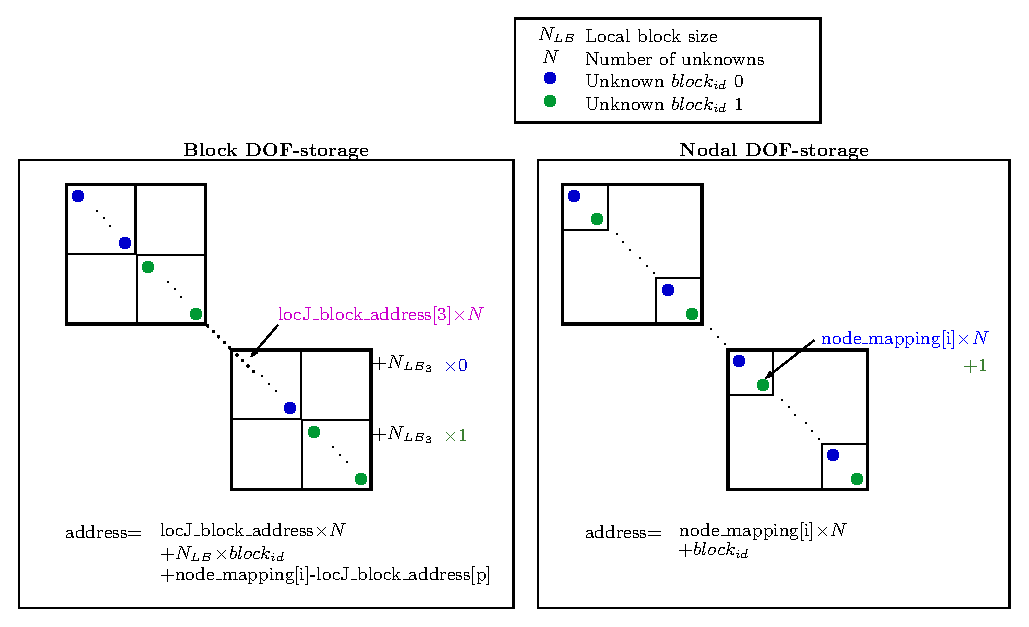
\includegraphics[width=1.0\linewidth]{Figures/DiscretizationComponentBlockCFEM}
\caption{Addressing scheme for multiblock unknowns with the CFEM discretization method.}
\label{fig:discretizationcomponentblockcfem}
\end{figure}



\newpage
\section{CFEM verification}
This section establishes a suite of test cases to verify the accurate implementation of the CFEM method. For each dimension we will restrict the domain $r \in [-1,1]$.

\subsection{Slab 1D}
Consider the one dimensional problem

\begin{equation*}
-\frac{\partial}{\partial x} \frac{\partial \phi}{\partial x} = 1 \quad \quad \forall x \in [-1,1]
\end{equation*}

We will apply different boundary conditions to test the implementation.

\subsubsection{Dirichlet boundary conditions}
We now consider the problem

\begin{equation*}
\begin{aligned}
-\frac{\partial}{\partial x} \frac{\partial \phi}{\partial x} = 1 \quad \quad \forall x \in [-1,1] \\
\phi(-1) = 1 \quad \quad \text{on } \partial \bOmega \\
\phi(1) = 1 \quad \quad \text{on } \partial \bOmega
\end{aligned}
\end{equation*}

which has the analytical solution

\begin{equation*}
\begin{aligned}
\phi(x) = -\frac{1}{2}x^2 + \frac{3}{2} \\
\end{aligned}
\end{equation*}

A comparison of the solutions is shown in Figure \ref{fig:Diffusion1a}. The comparison looks good.

\begin{figure}[H]
\centering
\includegraphics[width=0.8\linewidth]{Figures/Diffusion1a}
\caption{Comparison of CFEM solution to analytical solution.}
\label{fig:Diffusion1a}
\end{figure}

\subsubsection{Reflecting boundary condition}
Implementing a reflecting boundary condition cannot involve both boundaries being reflecting or else the system will be indeterminite. Therefore we will take the previous analytical solution and attempt to simulate the right half.

\begin{equation*}
\begin{aligned}
-\frac{\partial}{\partial x} \frac{\partial \phi}{\partial x} = 1 \quad \quad \forall x \in [-1,1] \\
\frac{\partial \phi}{\partial x}\biggr |_{x=0} = 0 \quad \quad \text{on } \partial \bOmega \\
\phi(1) = 1 \quad \quad \text{on } \partial \bOmega
\end{aligned}
\end{equation*}

The analytical solution is still

\begin{equation*}
\begin{aligned}
\phi(x) = -\frac{1}{2}x^2 + \frac{3}{2} \\
\end{aligned}
\end{equation*}

The results are shown in Figure \ref{fig:Diffusion1b} below.

\begin{figure}[H]
\centering
\includegraphics[width=0.8\linewidth]{Figures/Diffusion1b}
\caption{Comparison of CFEM solution to analytical solution using a reflecting boundary.}
\label{fig:Diffusion1b}
\end{figure}

\subsubsection{Vacuum boundary conditions}
For vacuum boundary conditions we deal with the following

\begin{equation*}
\begin{aligned}
-\frac{\partial}{\partial x} \frac{\partial \phi}{\partial x} = 1 \quad \quad \forall x \in [-1,1] \\
\frac{1}{4}\phi + \frac{1}{2}D \hat{n} \cdot \frac{\partial \phi}{\partial x} = 0 \quad \quad \text{on } \partial \bOmega \\
\end{aligned}
\end{equation*}

The results are shown in Figure \ref{fig:Diffusion1c}.

\begin{figure}[H]
\centering
\includegraphics[width=0.8\linewidth]{Figures/Diffusion1c}
\caption{Comparison of CFEM solution to analytical solution using vacuum boundary conditions.}
\label{fig:Diffusion1c}
\end{figure}

\newpage
\chead{DFEM}
\section{Modified Interior Penalty}
Instead of a Continuous Finite Element Method (CFEM) discretization, 
where the solution is defined on nodes, the Discontinuous Finite Element
Method (DFEM) stores values per cell. More specifically, using Piecewise
Linear (PWL) basis functions and trial functions, defines the solution per cell 
node. The complication with using this formulation is then that the 
connectivity between cells is not as easy to determine as it was for 
CFEM discretization.

The weak form of the diffusion equation is extended as can be observed 
in the paper by Ragusa, repeated here, the interior penalty method matrix takes on the form
\begin{equation*}
\begin{aligned}
a(\delta \phi,b_i) &= 
(\sigma_a \delta \phi, b_i)_{\mathcal{D}} + 
(D\nabla \delta \phi,\nabla b_i)_{\mathcal{D}} \\
&+ 
(\kappa^{MIP} \llbracket \delta \phi \rrbracket,\llbracket b_i \rrbracket)_f +
(\llbracket \delta \phi \rrbracket,\ldblbrace D \partial_n b_i \rdblbrace)_f +
(\ldblbrace D \partial_n \delta \phi \rdblbrace,\llbracket b_i \rrbracket)_f \\
&+
(\kappa^{M I P} \delta \phi, b_{i})_{\partial \mathcal{D}} -
\frac{1}{2}(\delta \phi, \mathrm{D} \partial_{n} b_{i})_{\partial \mathcal{D}}-
\frac{1}{2}(\mathrm{D} \partial_{n} \delta \phi, b_{i})_{\partial \mathcal{D}}
\end{aligned}
\end{equation*}
\newline
where the jump and average operators are defined across an interface as
\begin{equation*}
\begin{aligned}
\llbracket u \rrbracket &= u^+ - u^- \\
\ldblbrace u \rdblbrace &= \frac{1}{2}(u^+ + u^-)
\end{aligned}
\end{equation*}
\newline 
The definition of $\kappa^{MIP}$ is discussed in a later section.
The $\pm$ is associated with the sense the given cell has with the given 
face, i.e. if the face has the righthand-rule convention and consistency 
with the normal then the cell that has a negative sense to it is the 
cell to which this convention is consistent. For our purposes we will 
denote $cell^-$ as the ``current"-cell and $cell^+$ as the ``adjacent"-cell.
\newline 
\newline
Other notations used here are the volume integrals, $(F)_{\mathcal{D}}$, 
integration over interior faces $(F)_f$, and integration over face 
exterior faces $(F)_{\partial \mathcal{D}}$ on the boundary of the domain.
\newline 
\newline
To assemble the matrix entries using this formulation we can replace $\delta \phi$ with $b_j$ to find

\begin{equation*}
\begin{aligned}
a(b_j,b_i) &= 
(\sigma_a b_j, b_i)_{\mathcal{D}} + 
(D\nabla b_j,\nabla b_i)_{\mathcal{D}} \\
&+ 
(\kappa^{MIP} \llbracket b_j \rrbracket,\llbracket b_i \rrbracket)_f +
(\llbracket b_j \rrbracket,\ldblbrace D \partial_n b_i \rdblbrace)_f +
(\ldblbrace D \partial_n b_j \rdblbrace,\llbracket b_i \rrbracket)_f \\
&+
(\kappa^{M I P} b_j, b_{i})_{\partial \mathcal{D}} -
\frac{1}{2}(b_j, \mathrm{D} \partial_{n} b_{i})_{\partial \mathcal{D}}-
\frac{1}{2}(\mathrm{D} \partial_{n} b_j, b_{i})_{\partial \mathcal{D}}
\end{aligned}
\end{equation*}
\newline 
Let us now develop these terms part-by-part. Imagine 3 terms, corresponding to the terms that have
either $\llbracket \rrbracket$ or $\ldblbrace \rdblbrace$, which will be termed part A, B and C.

\newpage
\subsection{Part A}
Part A then becomes
\begin{equation*}
\begin{aligned}
(\kappa^{MIP} \llbracket b_j \rrbracket,\llbracket b_i \rrbracket)_f = 
\int_f \kappa^{MIP} \llbracket b_j \rrbracket,\llbracket b_i \rrbracket .dA
\end{aligned}
\end{equation*}
Now, for simplicity let us replace $\kappa^{MIP}$ with $K$ and only focus on the terms inside
the integral, part A now becomes

\begin{equation}
\begin{aligned}
&\quad \kappa^{MIP} \llbracket b_j \rrbracket,\llbracket b_i \rrbracket \\ 
&= K (b_j^+ - b_j^-)(b_i^+ - b_i^-) \\
&= K (b_i^+ - b_i^-) b_j^+ - K (b_i^+ - b_i^-) b_j^-  \\
&= K (b_i^+ - b_i^-) b_j^+ \quad + \Aboxed{K (b_i^- - b_i^+) b_j^-} .
\end{aligned}
\end{equation}
\newline 
The assembly of the interface terms into the matrix is a very complicated
 process. Each interface has to update each cell belonging to the 
 interface. This is further complicated by the nominal way in which the
 matrix is normally assembled, i.e. cell-by-cell. Fortunately, some 
 symmetry exists within the different parts as can be seen in part A above.
 The boxed portion in the above code is symmetric to the unboxed portion
 with respect to the cell with a negative sense to the face. In other words
 if we loop cell by cell and only execute the boxed portion, this will be
 equivalent to looping over the interfaces and updating both sides.

Given we computed $K$ we can now calculate the following on the interface
based on our current cell location ($cell^-$)

\begin{equation}
\begin{aligned}
& \quad (\kappa^{MIP} \llbracket b_j \rrbracket,\llbracket b_i \rrbracket)_{E_h^i} \\
&\text{for }i,j \text{ on current cell}\\
&\text{for }i^* \text{ on adjacent cell}\\
a_{i_rj_r} &= \biggr[ \kappa^{MIP} \int_{S_f} b_i.b_j.dA \biggr]_{cur-cell}\\
a_{i_r^*j_r} &= \biggr[ -\kappa^{MIP} \int_{S_f} b_{i^*}.b_j.dA \biggr]_{adj-cell},
\end{aligned}
\end{equation}

where $i_r$ and $j_r$ refers to the global matrix row and columns as 
mapped from the local matrices. The coding implementation for this is 
shown on the next page.
\newline
\newline
The implementation features a primary loop over trial space $i$ followed by a 
secondary loop over basis functions $j$. Since we are dealing only with the 
shape functions we loop over face dofs and map the face DOFs to cell DOFs using
the data \textbf{edge\_dof\_mappings}, developed during FE initialization. We
also use the ``interior penalty"-view of the cell to determine the matrix row
($ir$) corresponding to this cell's DOF-$i$. Since we are dealing with $b_i^*$ 
we also have to determine $i_r^*$, and hence we determine $i_{map}$ which is the
adjacent cell's DOF-$i$ index that corresponds to the current cell's DOF-$i$. 
The mapping of $i_{map}$ is then used with the adjacent cell's 
``interior penalty''-view to map to $i_r^*$. A similar procedure is applied to
the $b_j$ components but this time we are not dealing with indices on the adjacent
cell and therefore only $j_r$ is mapped. The values are inserted into global
matrix using PETSc's \textbf{MatSetValue} which need not refer to local values 
only.
\vspace{0.5cm}
\begin{lstlisting}[language=c++]
//========================= Assemble penalty terms
for (int fi=0; fi<num_face_dofs; fi++)
{
	int i  = fe_view->edge_dof_mappings[f][fi];
	int ir = cell_ip_view->MapDof(i);

	//Mapping face index to adj-cell
	int imap = MapCellDof(adj_cell,poly_cell->edges[f][fi]);
	int irstar = adj_ip_view->MapDof(imap);

	for (int fj=0; fj<2; fj++)
	{
		int j  = fe_view->edge_dof_mappings[f][fj];
		int jr = cell_ip_view->MapDof(j);

		double aij = kappa*fe_view->IntS_shapeI_shapeJ[f][i][j];

		MatSetValue(A,ir    ,jr, aij,ADD_VALUES);
		MatSetValue(A,irstar,jr,-aij,ADD_VALUES);
	}//for fj

}//for fi
\end{lstlisting}

\vspace{0.5cm}
\subsection{Part B}
Part B is 
\begin{equation*}
(\llbracket b_j \rrbracket,\ldblbrace D \partial_n b_i \rdblbrace)_f  =
\int_f \llbracket b_j \rrbracket,\ldblbrace D \partial_n b_i \rdblbrace .dA
\end{equation*}

Let us now expand the terms inside the integral

\begin{equation*}
\begin{aligned}
 &\llbracket b_j \rrbracket,\ldblbrace D \partial_n b_i \rdblbrace \\
 &= \frac{1}{2}\biggr(b_j^+ - b_j^-\biggr)\biggr(D^+\hat{n}\cdot\nabla b_i^+ + D^-\hat{n}\cdot\nabla b_i^-\biggr)\\
  &=\frac{1}{2}\biggr(D^+\hat{n}\cdot\nabla b_i^+ + D^-\hat{n}\cdot\nabla b_i^- \biggr)b_j^+
  - \frac{1}{2}\biggr(D^+\hat{n}\cdot\nabla b_i^+ + D^-\hat{n}\cdot\nabla b_i^- \biggr)b_j^-\\
 &=\frac{1}{2}\biggr(D^+\hat{n}\cdot\nabla b_i^+ + D^-\hat{n}\cdot\nabla b_i^-\biggr)b_j^+
 \Aboxed{
 - \frac{1}{2}\biggr(D^+\hat{n}\cdot\nabla b_i^+ + D^-\hat{n}\cdot\nabla b_i^-\biggr)b_j^-}
\end{aligned}
\end{equation*}
\newline
The blocked term in this equation is symmetric to the non-blocked terms with respect to the current cell and the adjacent cell. In other words, the normal ($\hat{n}$) in the blocked portion is with respect to the current cell ($cell^-$). When we flip the sign of all the $\pm$ denotations and set $\hat{n} = -\hat{n}$ then we obtain the non-blocked terms.
Some of the terms in the blocked portions can be combined with others so let us defer showing the code for that for now and proceed to part C.

\subsection{Part C}
Part C is
\begin{equation*}
(\ldblbrace D \partial_n b_j \rdblbrace,\llbracket b_i \rrbracket)_f  =
\int_f \ldblbrace D \partial_n b_j \rdblbrace,\llbracket b_i \rrbracket .dA
\end{equation*}

Let us now expand the terms inside the integral

\begin{equation*}
\begin{aligned}
 &\ldblbrace D \partial_n b_j \rdblbrace,\llbracket b_i \rrbracket \\
 &= \frac{1}{2}\biggr(b_i^+ - b_i^-\biggr)\biggr(D^+\hat{n}\cdot\nabla b_j^+ + D^-\hat{n}\cdot\nabla b_j^-\biggr)\\
 &= \frac{1}{2}\biggr(D^+\hat{n}\cdot\nabla b_j^+ + D^-\hat{n}\cdot\nabla b_j^-\biggr)b_i^+
- \frac{1}{2}\biggr(D^+\hat{n}\cdot\nabla b_j^+ + D^-\hat{n}\cdot\nabla b_j^-\biggr)b_i^-\\
 &= \frac{1}{2}\biggr(D^+\hat{n}\cdot\nabla b_j^+ + D^-\hat{n}\cdot\nabla b_j^-\biggr)b_i^+
 \Aboxed{
- \frac{1}{2}\biggr(D^+\hat{n}\cdot\nabla b_j^+ + D^-\hat{n}\cdot\nabla b_j^-\biggr)b_i^-}
\end{aligned}
\end{equation*}
\newline
Again the same symmetry applies as with part B (i.e. flipping the denotations and the signs on the normals).

\subsection{Assembling B and C}
We first look at the blocked parts of B and C together

\begin{equation*}
\begin{aligned}
 &\Aboxed{
  - \frac{1}{2}\biggr(D^+\hat{n}\cdot\nabla b_i^+ + D^-\hat{n}\cdot\nabla b_i^-\biggr)b_j^-} \quad
 \Aboxed{
- \frac{1}{2}\biggr(D^+\hat{n}\cdot\nabla b_j^+ + D^-\hat{n}\cdot\nabla b_j^-\biggr)b_i^-}\\
\end{aligned}
\end{equation*}

\begin{equation*}
\begin{aligned}
&=
- \frac{1}{2} b_j^- D^+\hat{n}\cdot\nabla b_i^+ \quad
- \frac{1}{2} b_j^- D^-\hat{n}\cdot\nabla b_i^- \quad
- \frac{1}{2} b_i^- D^+\hat{n}\cdot\nabla b_j^+ \quad
- \frac{1}{2} b_i^- D^-\hat{n}\cdot\nabla b_j^- 
\end{aligned}
\end{equation*}
\newline
We now reshuffle the terms here after first noting that the second and last terms are the transpose of each other as well as the first and third.

\begin{equation*}
\begin{aligned}
&=
- \frac{1}{2} b_j^- D^-\hat{n}\cdot\nabla b_i^- \quad
- \frac{1}{2} b_i^- D^-\hat{n}\cdot\nabla b_j^- \quad
- \frac{1}{2} b_j^- D^+\hat{n}\cdot\nabla b_i^+ \quad
- \frac{1}{2} b_i^- D^+\hat{n}\cdot\nabla b_j^+ 
\end{aligned}
\end{equation*}
\newline
We now reintroduce the surface integrals

\begin{equation*}
\begin{aligned}
&\int_f \biggr[
- \frac{1}{2} b_j^- D^-\hat{n}\cdot\nabla b_i^- \quad
- \frac{1}{2} b_i^- D^-\hat{n}\cdot\nabla b_j^- \quad
- \frac{1}{2} b_j^- D^+\hat{n}\cdot\nabla b_i^+ \quad
- \frac{1}{2} b_i^- D^+\hat{n}\cdot\nabla b_j^+ 
\biggr].dA \\
&=- \frac{1}{2} D^-\hat{n} \cdot \int_f \biggr(
b_j^- \cdot\nabla b_i^- +
b_i^- \cdot\nabla b_j^-
\biggr).dA \quad
- \frac{1}{2} D^+\hat{n}\cdot  \int_f \biggr(
b_j^- \cdot\nabla b_i^+
\biggr).dA \quad
- \frac{1}{2} D^+\hat{n}\cdot  \int_f \biggr(
b_i^- \cdot\nabla b_j^+
\biggr).dA
\end{aligned}
\end{equation*}
\newline
Theoretically the two right hand integrals could have been lumped in a similar fashion to the left-most integral, however, this segregation proved useful for efficiency in the looping structure with minimal mapping. We therefore have the following three equations to implement

\begin{equation}
a_{i_r,j_r} = 
- \frac{1}{2} D^-\hat{n} \cdot \int_f \biggr(
b_j^- \cdot\nabla b_i^- +
b_i^- \cdot\nabla b_j^-
\biggr).dA
\end{equation}

\begin{equation}
a_{i_r^*,j_r} = 
- \frac{1}{2} D^+\hat{n}\cdot  \int_f \biggr(
b_j^- \cdot\nabla b_i^+
\biggr).dA
\end{equation}

\begin{equation}
a_{i_r,j_r^*} = 
- \frac{1}{2} D^+\hat{n}\cdot  \int_f \biggr(
b_i^- \cdot\nabla b_j^+
\biggr).dA
\end{equation}
\newline
The coding implementation is shown below:

\vspace{0.5cm}
\begin{lstlisting}[language=c++]
// -Di^- bj^- and
// -Dj^- bi^-
for (int i=0; i<fe_view->dofs; i++)
{
  int ir = cell_ip_view->MapDof(i);

  for (int j=0; j<fe_view->dofs; j++)
  {
    int jr = cell_ip_view->MapDof(j);

    double gij =
      n.Dot(fe_view->IntS_shapeI_gradshapeJ[f][i][j] +
            fe_view->IntS_shapeI_gradshapeJ[f][j][i]);
    double aij = -0.5*diffCoeff*gij;

    MatSetValue(A,ir,jr,aij,ADD_VALUES);
  }//for j
}//for i
\end{lstlisting}

\vspace{0.25cm}
\begin{lstlisting}[language=c++]
// - Di^+ bj^-
for (int imap=0; imap<adj_fe_view->dofs; imap++)
{
  int irmap = adj_ip_view->MapDof(imap);

  for (int fj=0; fj<num_face_dofs; fj++)
  {
    int jmap  = MapCellDof(adj_cell,poly_cell->edges[f][fj]);
    int j     = MapCellDof(poly_cell,poly_cell->edges[f][fj]);
    int jr    = cell_ip_view->MapDof(j);

    double gij =
      n.Dot(adj_fe_view->IntS_shapeI_gradshapeJ[fmap][jmap][imap]);
    double aij = -0.5*diffCoeff*gij;

    MatSetValue(A,irmap,jr,aij,ADD_VALUES);
  }//for j
}//for i
\end{lstlisting}

\vspace{0.25cm}
\begin{lstlisting}[language=c++]
// - Dj^+ bi^-
for (int jmap=0; jmap<adj_fe_view->dofs; jmap++)
{
  int jrmap = adj_ip_view->MapDof(jmap);

  for (int fi=0; fi<num_face_dofs; fi++)
  {
    int imap  = MapCellDof(adj_cell,poly_cell->edges[f][fi]);
    int i     = MapCellDof(poly_cell,poly_cell->edges[f][fi]);
    int ir    = cell_ip_view->MapDof(i);

    double gij =
      n.Dot(adj_fe_view->IntS_shapeI_gradshapeJ[fmap][imap][jmap]);
    double aij = -0.5*diffCoeff*gij;

    MatSetValue(A,ir,jrmap,aij,ADD_VALUES);
  }//for j
}//for i
\end{lstlisting}

\newpage
\chead{References}
\begin{thebibliography}{1}
    
    \bibitem{MMD} Moukalled F., Mangani L., Darwish M., {\em The Finite Volume Method in Computational Fluid Dynamics - An Advanced Introduction with OpenFOAM and Matlab}, Springer, 2016.
    
    \bibitem{Sezai} Sezai I., {\em Implementation of boundary conditions in pressure-based finite volume methods on unstructured grids}, Numerical Heat Transfer, Part B: Fundamentals, 2017
    
    \bibitem{blender} {\em Blender - a 3D modelling and rendering package}, Blender Online Community, Blender Foundation, Blender Institute, Amsterdam, 2018
    
    \bibitem{delaunay} Cheng et al, {\em Delaunay Mesh Generation}, Chapman \& Hall/CRC Computer \& Information Science Series, 2013
    
    
\end{thebibliography}





\end{document}